

\subsection{Analysing the $2$-Player sub-game}
\label{subsec:2_player_subgame_piratas_doidos}

By hypothesis, the way we set up our system may originate different results, so when we have a $3$ player system, we will try to analyse the sub-game with $2$ players taking into account the original system. In the classical version of the Pirate Game, the problem with $2$ players is equivalent to a sub-problem with $2$ players of a problem with more players where previous captains are killed. 

\begin{table}
\begin{center}
\begin{tabular}{cc}
  a)\putindeepbox[7pt]{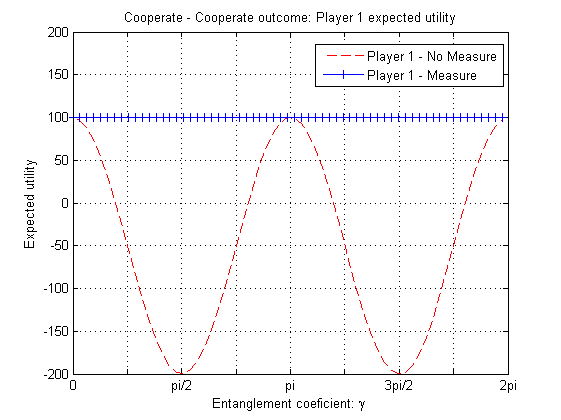
\includegraphics[scale=0.48]{compareluders/CC1.PNG}}
    & b)\putindeepbox[7pt]{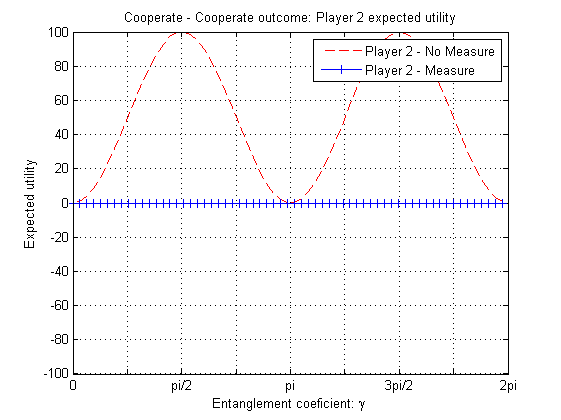
\includegraphics[scale=0.48]{compareluders/CC2.PNG}} \\
  c)\putindeepbox[7pt]{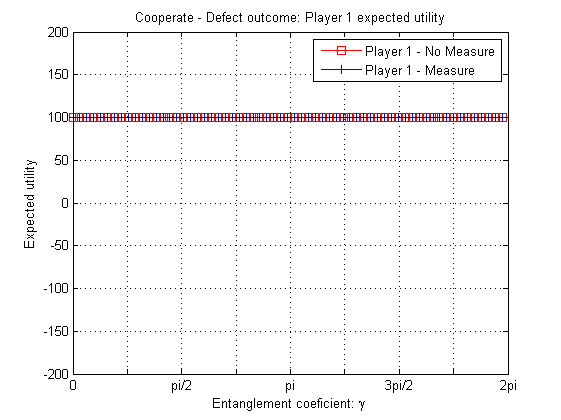
\includegraphics[scale=0.48]{compareluders/CD1.PNG}}
    & d)\putindeepbox[7pt]{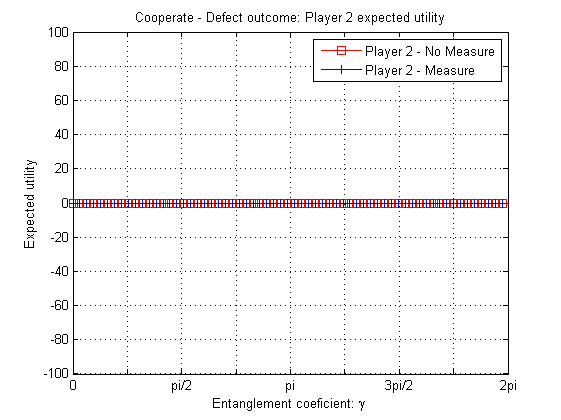
\includegraphics[scale=0.48]{compareluders/CD2.PNG}} \\
  e)\putindeepbox[7pt]{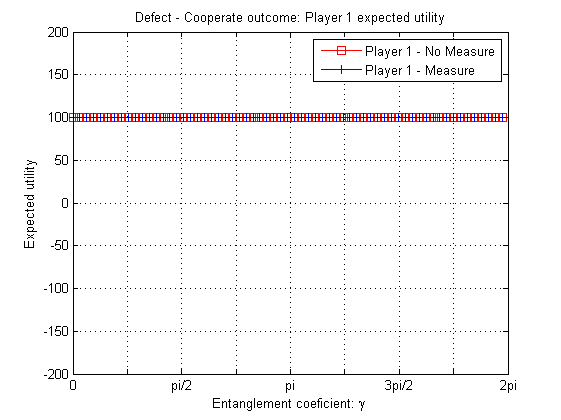
\includegraphics[scale=0.46]{compareluders/DC1.PNG}}
    & f)\putindeepbox[7pt]{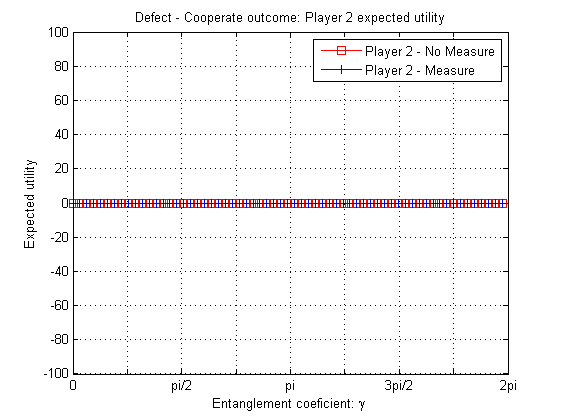
\includegraphics[scale=0.48]{compareluders/DC2.PNG}} \\
  g)\putindeepbox[7pt]{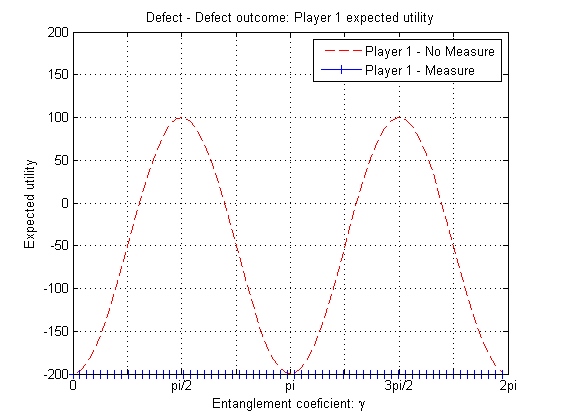
\includegraphics[scale=0.46]{compareluders/DD1.PNG}}
    & h)\putindeepbox[7pt]{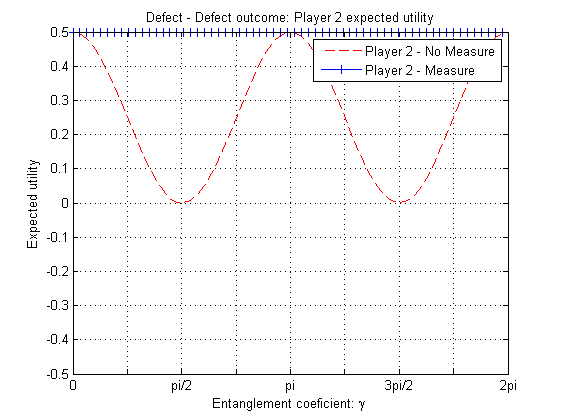
\includegraphics[scale=0.48]{compareluders/DD2.PNG}} \\
\end{tabular}
\caption{Comparison of the expected utilities when measuring and not measuring between steps 1 and 2 of a 3 player game (the player 1 will be the player 2 in the 3 player game, and the player 2 will be the player 3 in the 3 game situation).}
\label{tab:luderscomp}
\end{center}
 \end{table}



We set up a system with $3$ players and in the step $1$ the three players chose the operators $o_{10},o_{21},o_{31}$ producing the outcome $CDD$, the initial proposal for the gold coin division will be $(100, 0, 0)$. 

To analyse the step $2$, or the sub-game with $2$ pirates,  the system will be kept in the initial dimension ($\mathcal{H}^{3}$), because of the following reasons: if we have entangled states, they won't be are separable; There may be various mappings in a lower dimension that fit the higher dimension composition. This means that the previous highest ranking player will no longer have access to the voting operators, instead she will use invariably a symmetric coin operator $H$.

In one situation we will use the L\"{u}der's Rule, after the voting. This is the equivalent of performing a measurement on the system after the first round \ref{fig:pg_architecture3players_2measure}. In the other situation the two players will act on step $2$, as in Figure \ref{fig:pg_architecture3players_2nomeasure}. The results for this experiment (Table \ref{tab:luderscomp}), allow us to conclude that not measuring the system affects the expected utilities for the players in two of the four possible analysed outcomes. 

In this case the act of measuring leaves us with the same utility results one would get in a classic situation with $2$ players game, the equilibrium here is $CD$ outcome. 

Without the intermediate measuring step the outcome will depend on the $\gamma$ - the initial coefficient used to set up the system. For example:

\begin{itemize}
\item $\gamma = 0$, we have the same results as in the original problem. The Nash equilibrium is unique and it is $CD$.
\item $\gamma = \frac{\pi}{2}$, the equilibrium is $DC$, as the payoffs for the $CC$ outcome are $(-200, 0.5)$, and the outcome $DD$ will present $(100, 0)$ for the expected utilities of the players.
\item $\gamma = \frac{\pi}{4}$, all possible outcomes will be Nash equilibria. As we can see in Table \ref{tab:hate_myself}, no player can improve her payoff by unilaterally changing her strategy.



\end{itemize}

\begin{center}
\begin{table}
\begin{centering}
\begin{tabular}{ccc}
\hline 
 $\gamma = \frac{\pi}{4}$ & Player 2: C & Player 2: D\tabularnewline
\hline 
Player 1: C & (-50, 50.25) & (100, 0)\tabularnewline
Player 1: D & (100, 0) & (-50, 50.25)\tabularnewline
\hline 
\end{tabular}
\par\end{centering}

\caption{Normal form representation of the second step in a 3 player game with an entanglement coefficient of $\frac{\pi}{4}$, where there isn't an intermediate measuring. }
\label{tab:hate_myself}
\end{table}
\end{center}
